
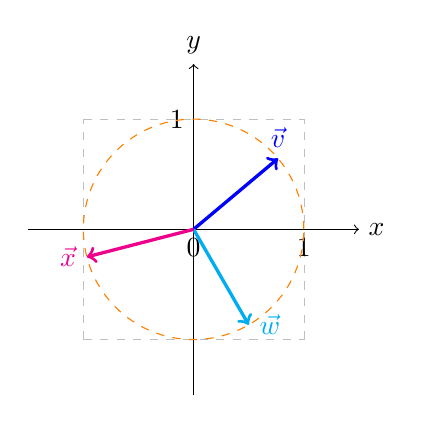
\begin{tikzpicture}[scale=1.4]
    \draw[step=1,help lines, dashed,lightgray] (-1,-1) grid (1,1);
    %draw axis value
    \foreach \x in {0,1}
        {%
            \draw (\x,0) -- (\x,0) node [below] {$\x$};
        }
    \foreach \y in {1}
        {%
            \draw (0,\y) -- (0,\y) node [left] {$\y$};
        }
    %draw lines
    \draw [->] (-1.5,0) -- (1.5,0) node[right]{$x$};
    \draw [->] (0,-1.5) -- (0,1.5) node[above]{$y$};
    \draw [->,blue,very thick] (0,0) -- (\fpeval{cos(40/180*pi)},\fpeval{sin(40/180*pi)}) node[above]{$\vec{v}$};
    \draw [->,cyan,very thick] (0,0) -- (0.5,-0.8660) node[right]{$\vec{w}$};
    \draw [->,magenta,very thick] (0,0) -- (-0.9682,-0.25) node[left]{$\vec{x}$};
    \draw (0,0) [dashed,orange] circle (1);
\end{tikzpicture}
\captionof{figure}{{\footnotesize $(\|\vec{v}\|=\|\vec{w}\|=\|\vec{x}\|=1)\in\mathbb{R}^2$}}
\label{fig:vector-and-vector-operation-d19}